% !TEX encoding = UTF-8 Unicode
% !TEX TS-program = xelatex
\begin{QUESTIONS}
    \begin{QUESTION}
        \begin{ExamInfo}{95}{學測}{單選}{1}
        \end{ExamInfo}
        \begin{ExamAnsRateInfo}{73}{97}{75}{47}
        \end{ExamAnsRateInfo}
        \begin{QBODY}
            設一元二次整係數方程式 $ax^2 + bx + c = 0$ 有一根為 $4 + 3i$。 若將此方程式的兩根與原點在複數平面上標出,則此三點所圍成的三角形面積為 
			\begin{QOPS} 
				\QOP 5 
				\QOP 6 
				\QOP 12 
				\QOP 16
				\QOP 24
			\end{QOPS}
        \end{QBODY}
        \begin{QFROMS}
        \end{QFROMS}
        \begin{QTAGS}\QTAG{B5C2-3複數的幾何意義}\QTAG{B5C2三角函數II}\QTAG{面積}\end{QTAGS}
        \begin{QANS}
            (5)
        \end{QANS}
        \begin{QSOLLIST}
        \end{QSOLLIST}
        \begin{QEMPTYSPACE}
        \end{QEMPTYSPACE}
    \end{QUESTION}
    \begin{QUESTION}
        \begin{ExamInfo}{95}{學測}{單選}{2}
        \end{ExamInfo}
        \begin{ExamAnsRateInfo}{40}{73}{38}{9}
        \end{ExamAnsRateInfo}
        \begin{QBODY}
            在右圖的棋盤方格中,隨機任意取兩個格子。選出的兩個格子不在同行(有無同列無所謂)的機率為
			\begin{QOPS} 
				\QOP $\frac{1}{20}$ 
				\QOP $\frac{1}{4}$ 
				\QOP $\frac{3}{4}$
				\QOP $\frac{3}{5}$ 
				\QOP $\frac{4}{5}$
			\end{QOPS}
			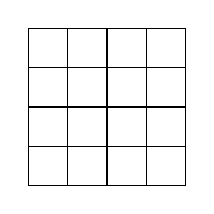
\begin{tikzpicture}[scale=.5]
				\foreach \y in {0,1,2,3,4}{
						\draw (0,\y) to (4,\y);
						\draw (\y,0) to (\y,4);
				}
			\end{tikzpicture}
        \end{QBODY}
        \begin{QFROMS}
        \end{QFROMS}
        \begin{QTAGS}\QTAG{B2C3機率}\QTAG{B2C3-2機率的定義與性質}\end{QTAGS}
        \begin{QANS}
            (4)
        \end{QANS}
        \begin{QSOLLIST}
        \end{QSOLLIST}
        \begin{QEMPTYSPACE}
        \end{QEMPTYSPACE}
    \end{QUESTION}
    \begin{QUESTION}
        \begin{ExamInfo}{95}{學測}{單選}{3}
        \end{ExamInfo}
        \begin{ExamAnsRateInfo}{52}{88}{46}{22}
        \end{ExamAnsRateInfo}
        \begin{QBODY}
            右圖是由三個直角三角形堆疊而成的圖形,且 $\overline{OD} = 8$ 。
			問:直角三角形 $OAB$ 的高 $\overline{AB}$ 為何?
			\begin{QOPS} 
				\QOP $1$
				\QOP $\sqrt{6}-\sqrt{2}$ 
				\QOP $\sqrt{7}-1$ 
				\QOP $\sqrt{3}$ 
				\QOP $2$
			\end{QOPS}
			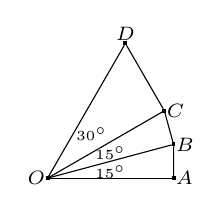
\begin{tikzpicture}[inner sep=0pt,scale=.8]\scriptsize
				\node (O) at (0,0) [label=180:$O$,draw,fill]{}; 
				\node (A) at (2,0) [label=0:$A$,draw,fill]{}; 
				\node (B) at (15:2.07) [label=0:$B$,draw,fill]{}; 
				\node (C) at (30:2.14) [label=0:$C$,draw,fill]{}; 
				\node (D) at (60:2.47) [label=90:$D$,draw,fill]{}; 
				\draw (0,0) to (A);
				\draw (0,0) to (B);
				\draw (0,0) to (C);
				\draw (0,0) to (D);
				\draw (A) to (B);
				\draw (B) to (C);
				\draw (C) to (D);
				\tiny
				\node at (.7,.7) {$30^\circ$};
				\node at (1,.4) {$15^\circ$};
				\node at (1,.1) {$15^\circ$};
			\end{tikzpicture}
        \end{QBODY}
        \begin{QFROMS}
        \end{QFROMS}
        \begin{QTAGS}\QTAG{B3C1三角}\end{QTAGS}
        \begin{QANS}
            (4)
        \end{QANS}
        \begin{QSOLLIST}
        \end{QSOLLIST}
        \begin{QEMPTYSPACE}
        \end{QEMPTYSPACE}
    \end{QUESTION}
    \begin{QUESTION}
        \begin{ExamInfo}{95}{學測}{單選}{4}
        \end{ExamInfo}
        \begin{ExamAnsRateInfo}{34}{67}{23}{12}
        \end{ExamAnsRateInfo}
        \begin{QBODY}
            下列哪一個數值最接近 $-\sqrt{2}$ ? 
			\begin{QOPS} 
				\QOP $\sqrt{3}\cos{44^\circ}+ \sin{44^\circ}$ 
				\QOP $\sqrt{3}\cos{54^\circ}+ \sin{54^\circ}$ 
				\QOP $\sqrt{3}\cos{64^\circ} +\sin{64^\circ}$
				\QOP $\sqrt{3}\cos{74^\circ}+\sin{74^\circ}$
				\QOP $\sqrt{3}\cos{84^\circ}+i\sin{84^\circ}$
			\end{QOPS}
        \end{QBODY}
        \begin{QFROMS}
        \end{QFROMS}
        \begin{QTAGS}\QTAG{B3C1三角}\end{QTAGS}
        \begin{QANS}
            (4)
        \end{QANS}
        \begin{QSOLLIST}
        \end{QSOLLIST}
        \begin{QEMPTYSPACE}
        \end{QEMPTYSPACE}
    \end{QUESTION}
    \begin{QUESTION}
        \begin{ExamInfo}{95}{學測}{單選}{5}
        \end{ExamInfo}
        \begin{ExamAnsRateInfo}{24}{50}{15}{7}
        \end{ExamAnsRateInfo}
        \begin{QBODY}
            在養分充足的情況下,細菌的數量會以指數函數的方式成長,假設細菌 $A$ 的數量每兩個小時可以成長為兩倍,細菌 $B$ 的數量每三個小時可以成長為三倍。若養分充足且一開始兩種細菌的數量相等,則大約幾小時後細菌 $B$ 的數量除以細菌 $A$ 的數量最接近 10 ? 
			\begin{QOPS} 
				\QOP $24 $小時    
				\QOP $48 $小時    
				\QOP $69 $小時 
				\QOP $96 $小時    
				\QOP $117$ 小時
			\end{QOPS}
        \end{QBODY}
        \begin{QFROMS}
        \end{QFROMS}
        \begin{QTAGS}\QTAG{應用問題}\QTAG{B1C3指對數函數}\QTAG{B1C3-5指數與對數的應用}\end{QTAGS}
        \begin{QANS}
            (5)
        \end{QANS}
        \begin{QSOLLIST}
        \end{QSOLLIST}
        \begin{QEMPTYSPACE}
        \end{QEMPTYSPACE}
    \end{QUESTION}
\end{QUESTIONS}
\begin{QUESTIONS}
    \begin{QUESTION}
        \begin{ExamInfo}{95}{學測}{多選}{6}
        \end{ExamInfo}
        \begin{ExamAnsRateInfo}{15}{27}{8}{10}
        \end{ExamAnsRateInfo}
        \begin{QBODY}
            假設 $a, b, c$ 是三個正整數。若 25 是 $a$, $b$ 的最大公因數,且 $3,4,14$ 都是 $b,c$ 的公因數,則下列何者正確?
				\begin{QOPS} 
					\QOP $c$ 一定可以被 56 整除。 
					\QOP 若 $a \leq 100$,則 $a=25$。 
					\QOP $a, b, c$ 三個數的最大公因數是 25	的因數。
					\QOP $a,b,c$ 三個數的最小公倍數大於或等於 $25 \times 3 \times 4 \times 14$ 。
				\end{QOPS}
        \end{QBODY}
        \begin{QFROMS}
        \end{QFROMS}
        \begin{QTAGS}\QTAG{不是99課綱}\end{QTAGS}
        \begin{QANS}
            (2)(3)(4)
        \end{QANS}
        \begin{QSOLLIST}
        \end{QSOLLIST}
        \begin{QEMPTYSPACE}
        \end{QEMPTYSPACE}
    \end{QUESTION}
    \begin{QUESTION}
        \begin{ExamInfo}{95}{學測}{多選}{7}
        \end{ExamInfo}
        \begin{ExamAnsRateInfo}{47}{83}{44}{14}
        \end{ExamAnsRateInfo}
        \begin{QBODY}
            考慮坐標平面上所有滿足 $\sqrt{(x-2)^2 +y^2} + \sqrt{(x-2)^2 +(y+4)^2} =10$ 的點 $(x,y)$ 所成的圖形,下列敘述何者正確? 
			\begin{QOPS} 
				\QOP 此圖形為一橢圓。
				\QOP 此圖形為一雙曲線。 
				\QOP 此圖形的中心在 $(2,-2)$。
				\QOP 此圖形對稱於 $x-2=0$。    
				\QOP 此圖形有一頂點 $(2, 3)$ 。
			\end{QOPS}
        \end{QBODY}
        \begin{QFROMS}
        \end{QFROMS}
        \begin{QTAGS}\QTAG{B4C4-3雙曲線}\QTAG{B4C4二次曲線}\QTAG{B4C4-2橢圓}\QTAG{圖形}\end{QTAGS}
        \begin{QANS}
            (1)(3)(4)(5)
        \end{QANS}
        \begin{QSOLLIST}
        \end{QSOLLIST}
        \begin{QEMPTYSPACE}
        \end{QEMPTYSPACE}
    \end{QUESTION}
    \begin{QUESTION}
        \begin{ExamInfo}{95}{學測}{多選}{8}
        \end{ExamInfo}
        \begin{ExamAnsRateInfo}{38}{71}{33}{10}
        \end{ExamAnsRateInfo}
        \begin{QBODY}
            假設實數 $a_1$, $a_2$, $a_3$, $a_4$ 是一個等差數列,且滿足 $0<a_1 <2$ 及 $a_3 =4$。若定義 $b_n =2^{a_n}$ , 則以下哪些選項是對的?
		\begin{QOPS} 
			\QOP $b_1 ,b_2 ,b_3 ,b_4$ 是一個等比數列 
			\QOP $b_1 <b_{2}$     
			\QOP $b_2 >4$ 
			\QOP $b_4 > 32$
			\QOP $b_2 \times b_4 =256$
		\end{QOPS}
        \end{QBODY}
        \begin{QFROMS}
        \end{QFROMS}
        \begin{QTAGS}\QTAG{B1C3-3對數}\QTAG{等差數列}\QTAG{B2C1數列級數}\QTAG{等比數列}\QTAG{B2C1-1數列}\QTAG{跨章節試題}\QTAG{B1C3指對數函數}\end{QTAGS}
        \begin{QANS}
            (1)(2)(3)(4)(5)
        \end{QANS}
        \begin{QSOLLIST}
        \end{QSOLLIST}
        \begin{QEMPTYSPACE}
        \end{QEMPTYSPACE}
    \end{QUESTION}
    \begin{QUESTION}
        \begin{ExamInfo}{95}{學測}{多選}{9}
        \end{ExamInfo}
        \begin{ExamAnsRateInfo}{38}{71}{30}{13}
        \end{ExamAnsRateInfo}
        \begin{QBODY}
            學生練習計算三次多項式 $f (x)$ 除以一次多項式 $g(x)$ 的餘式。
			已知 $f (x)$ 的三次項係數為 3, 一次項係數為 2。
			甲生在計算時把 $f(x)$ 的三次項係數錯看成 2 (其它係數沒看錯),
			乙生在計算時把 $f (x)$ 的一次項係數錯看成 $-2$ (其它係數沒看錯)。
			而甲生和乙生算出來的餘式剛好一樣。試問 $g(x)$ 可能等於以下哪些一次式?

			\begin{QOPSINONELINE} 
				\QOP $x$    \QOP $x-1$    \QOP $x-2$    \QOP $x+1$    \QOP $x+2$
			\end{QOPSINONELINE}
        \end{QBODY}
        \begin{QFROMS}
        \end{QFROMS}
        \begin{QTAGS}\QTAG{一次多項式}\QTAG{B1C2多項式函數}\QTAG{多項式除法}\QTAG{B1C2-2多項式的運算與應用}\end{QTAGS}
        \begin{QANS}
            (1)(3)(5)
        \end{QANS}
        \begin{QSOLLIST}
        \end{QSOLLIST}
        \begin{QEMPTYSPACE}
        \end{QEMPTYSPACE}
    \end{QUESTION}
    \begin{QUESTION}
        \begin{ExamInfo}{95}{學測}{多選}{10}
        \end{ExamInfo}
        \begin{ExamAnsRateInfo}{27}{48}{23}{10}
        \end{ExamAnsRateInfo}
        \begin{QBODY}
            下圖是根據 100 名婦女的體重所 作出的直方圖(圖中百分比數字代表各體重區間的相對次數,其中各區間不包含左端點而包含右端點)。該 100 名婦女體重的平均數 為 55 公斤,標準差為 12.5 公 斤。曲線 $N$ 代表一常態分佈,其平均數與標準差與樣本值相同。在此樣本中,若定義「體重過重」的標準為體重超過樣本平均數 2 個標準差以上(即體重超過 80 公斤以上),則下列敘述哪些正確? 
			\begin{QOPS} 
				\QOP 曲線 $N$ (常態分佈)中,在 55 公斤以上所佔的比例約為 $50\%$。 
				\QOP 曲線 $N$ (常態分佈)中,在 80 公斤以上所佔的比例約為 $2.5\%$ 。  
				\QOP 該樣本中,體重的中位數大於 55 公斤。 
				\QOP 該樣本中,體重的第一四分位數大於 45 公斤。 
				\QOP 該樣本中,「體重過重」(體重超過 80 公斤以上)的比例大於或等於 $5\%$。
			\end{QOPS}
			
			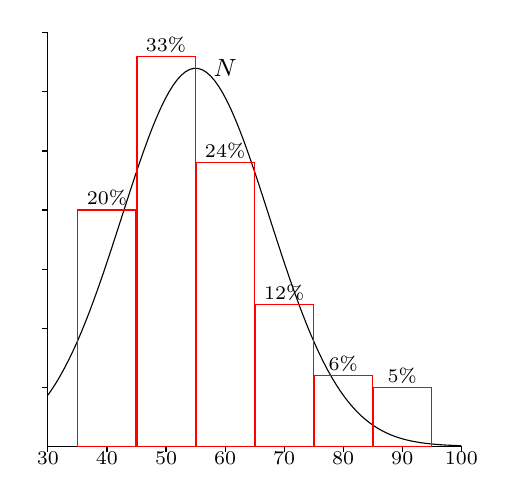
\begin{tikzpicture}[xscale=.75,yscale=.15]
				\node at (6,32) {\small $N$};
				\draw[domain=3:10,samples=100] plot (\x,{32*exp(-(\x-5.5)*(\x-5.5)/3.125)}) {};
				\begin{scope}[ybar]
				\draw (3,0) to (10,0);
				\draw (3,0) to(3,35);
				\foreach \i in {5,10,...,35}{
						\draw (3,\i) to (2.9,\i);
				}
				\foreach \i in {30,40,50,...,100}{
						\node at (0.1*\i,-1) {\scriptsize \i};
						\draw (0.1*\i,0) to (0.1*\i,-.5);
				}
				\foreach \i/\j in {40/20,50/33,60/24,70/12,80/6,90/5}{
						\node at (0.1*\i,\j+1) {\scriptsize \j $\%$};
				}
				\draw[color=red,bar width=28pt]
					plot coordinates{(4,20) (5,33) (6,24) (7,12) (8,6) (9,5) };
				\end{scope}
			\end{tikzpicture}
        \end{QBODY}
        \begin{QFROMS}
        \end{QFROMS}
        \begin{QTAGS}\QTAG{B5C1機率與統計}\end{QTAGS}
        \begin{QANS}
            (1)(2)(4)(5)
        \end{QANS}
        \begin{QSOLLIST}
        \end{QSOLLIST}
        \begin{QEMPTYSPACE}
        \end{QEMPTYSPACE}
    \end{QUESTION}
    \begin{QUESTION}
        \begin{ExamInfo}{95}{學測}{多選}{11}
        \end{ExamInfo}
        \begin{ExamAnsRateInfo}{76}{98}{89}{41}
        \end{ExamAnsRateInfo}
        \begin{QBODY}
            將正整數 18 分解成兩個正整數的乘積有 $1\times 18$ , $2\times 9$, $3\times 6$ 三種,又 $3 \times 6$ 是這三種分解中,兩數的差最小的,我們稱 $3 \times 6$ 為 18 的最佳分解。當 $p\times q (p \leq q)$ 是正整數 $n$ 的最佳分解時,我們規定函數 $F(n)=\frac{p}{q}$,例如 $F(18)=\frac{3}{6}=\frac{1}{2}$。
			下列有關函數 $F(n)$ 的敘述,何者正確? 
			\begin{QOPS} 
				\QOP $F(4) =1$    \QOP $F(24)=\frac{3}{8}$ 
				\QOP $F(27)=\frac{1}{3}$ 
				\QOP 若 $n$ 是一個質數,則 $F(n)=\frac{1}{n}$ 
				\QOP 若 $n$ 是一個完全平方數,則 $F(n) =1$。
			\end{QOPS}
        \end{QBODY}
        \begin{QFROMS}
        \end{QFROMS}
        \begin{QTAGS}\QTAG{不是99課綱}\end{QTAGS}
        \begin{QANS}
            (1)(3)(4)(5)
        \end{QANS}
        \begin{QSOLLIST}
        \end{QSOLLIST}
        \begin{QEMPTYSPACE}
        \end{QEMPTYSPACE}
    \end{QUESTION}
\end{QUESTIONS}
\begin{QUESTIONS}
    \begin{QUESTION}
        \begin{ExamInfo}{95}{學測}{填充}{A}
        \end{ExamInfo}
        \begin{ExamAnsRateInfo}{44}{80}{44}{8}
        \end{ExamAnsRateInfo}
        \begin{QBODY}
            抽樣調查某地區 1000 個有兩個小孩的家庭,得到如下數據,其中 (男,女) 代表第一個小孩是男孩而第二個小孩是女生的家庭,餘類推。由此數據可估計該地區有兩個小孩家庭的男、女孩性別比約為 $\TCNBOX{\TCN\TCN\TCN}:100 $(四捨五入至整數位)。
        \end{QBODY}
        \begin{QFROMS}
        \end{QFROMS}
        \begin{QTAGS}\QTAG{B5C1機率與統計}\QTAG{B5C1-3抽樣與統計推論}\end{QTAGS}
        \begin{QANS}
            $105$
        \end{QANS}
        \begin{QSOLLIST}
        \end{QSOLLIST}
        \begin{QEMPTYSPACE}
        \end{QEMPTYSPACE}
    \end{QUESTION}
    \begin{QUESTION}
        \begin{ExamInfo}{95}{學測}{填充}{B}
        \end{ExamInfo}
        \begin{ExamAnsRateInfo}{33}{77}{21}{1}
        \end{ExamAnsRateInfo}
        \begin{QBODY}
            右圖為一正立方體, 若 $M$ 在線段 $\overline{AB}$ 上,$\overline{BM} = 2\overline{AM}$, $N$ 為線段 $\overline{BC}$ 之中點,則 $\cos \angle MON = \TCNBOX{\FR{\TCN\sqrt{\TCN\TCN}}{\TCN\TCN}}$ 。(分數要化成最簡分數)
		
			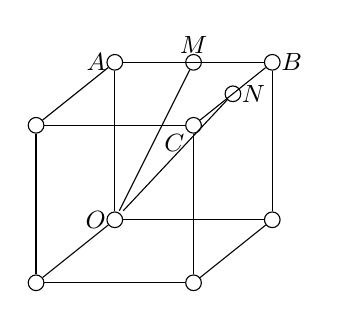
\begin{tikzpicture}
				\begin{scope}
				\small
				\node (vO) at (0,0) {};
				\tikzstyle{vnode}=[draw,circle,inner sep =2pt];
				\node[vnode] (v000) at (0,0) {};
				\node[anchor =east] (t000) at (v000) {$O$};
				%\fill [red] ($(a) + 1/3*(1cm,0)$) circle (2pt);
				\node[vnode] (v001) at (0,2) {$$};
				\node[anchor =east] (t000) at (v001) {$A$};
				\node[vnode] (v011) at (2,2) {$$};
				\node[anchor =west] (t011) at (v011) {$B$};
				\node[vnode] (v010) at (2,0) {$$};
				\node[anchor =west] (t010) at (v010) {$$};
				\node[vnode] (v100) at (-1.0,-.8) {$$};
				\node[anchor =west] (t100) at (v100) {$$};
				\node[vnode] (v101) at (-1.0,1.2) {$$};
				\node[anchor =west] (t101) at (v101) {$$};
				\node[vnode] (v111) at (1.0,1.2) {$$};
				\node[anchor =north east] (t111) at (v111) {$C$};
				\node[vnode] (v110) at (1.0,-0.8) {$$};
				\node[anchor =west] (t110) at (v110) {$$};
				\node[vnode] (vM) at (1,2) {$$};
				\node[anchor =south] (tM) at (vM) {$M$};
				\node[vnode] (vN) at (1.5,1.6) {$$};
				\node[anchor =west] (tN) at (vN) {$N$};
				\draw (vM) to[dashed] (vO);
				\draw (vN) to[dashed] (vO);
				\foreach \i in {01,10,11}{
						\draw (v0\i) to (v1\i);
						\draw (v\i  0) to (v\i 1);
				}
				\draw (v000) to[dashed] (v100);
				\draw (v000) to[dashed] (v010);
				\draw (v000) to[dashed] (v001);
				\draw (v001) to (v011);
				\draw (v100) to (v110);
				\draw (v101) to (v111);
				\end{scope}
			\end{tikzpicture}
        \end{QBODY}
        \begin{QFROMS}
        \end{QFROMS}
        \begin{QTAGS}\QTAG{B4C1-3空間向量的內積}\QTAG{B4C1空間向量}\end{QTAGS}
        \begin{QANS}
            $\frac{4\sqrt{10}}{15}$
        \end{QANS}
        \begin{QSOLLIST}
        \end{QSOLLIST}
        \begin{QEMPTYSPACE}
        \end{QEMPTYSPACE}
    \end{QUESTION}
    \begin{QUESTION}
        \begin{ExamInfo}{95}{學測}{填充}{C}
        \end{ExamInfo}
        \begin{ExamAnsRateInfo}{49}{88}{50}{9}
        \end{ExamAnsRateInfo}
        \begin{QBODY}
            給定平面上三點 $(-6, -2)$, $(2, -1)$, $(1, 2)$。若有第四點和此三點形成一菱形(四邊長皆相等),則第四點的坐標為 $\TCNBOX{(\TCN,\TCN)}$ 。
        \end{QBODY}
        \begin{QFROMS}
        \end{QFROMS}
        \begin{QTAGS}\QTAG{線性組合}\QTAG{B3C3-1平面向量的表示法}\QTAG{B3C3平面向量}\end{QTAGS}
        \begin{QANS}
            $(9,3)$
        \end{QANS}
        \begin{QSOLLIST}
        \end{QSOLLIST}
        \begin{QEMPTYSPACE}
        \end{QEMPTYSPACE}
    \end{QUESTION}
    \begin{QUESTION}
        \begin{ExamInfo}{95}{學測}{填充}{D}
        \end{ExamInfo}
        \begin{ExamAnsRateInfo}{34}{72}{26}{4}
        \end{ExamAnsRateInfo}
        \begin{QBODY}
            $ABCD$ 為圓內接四邊形,若 $\angle DBC = 30 ^\circ$, $\angle ABD = 45^\circ$, $\overline{CD}=6$,則線段 $\overline{AD}= \TCNBOX{\sqrt{\TCN\TCN}}$ 。
        \end{QBODY}
        \begin{QFROMS}
        \end{QFROMS}
        \begin{QTAGS}\QTAG{餘弦定理}\QTAG{B3C1-3正弦定理與餘弦定理}\QTAG{B3C1三角}\QTAG{正弦定理}\end{QTAGS}
        \begin{QANS}
            $\sqrt{72}$
        \end{QANS}
        \begin{QSOLLIST}
        \end{QSOLLIST}
        \begin{QEMPTYSPACE}
        \end{QEMPTYSPACE}
    \end{QUESTION}
    \begin{QUESTION}
        \begin{ExamInfo}{95}{學測}{填充}{E}
        \end{ExamInfo}
        \begin{ExamAnsRateInfo}{68}{89}{75}{40}
        \end{ExamAnsRateInfo}
        \begin{QBODY}
            新新鞋店為與同業進行促銷戰,推出「第二雙不用錢:買一送一」的活動。該鞋店共有八款 鞋可供選擇,其價格如下:規定所送的鞋之價格一定少於所買的價格(例如:買一個「丁」款鞋,可送甲、乙兩款鞋 之一)。若有一位新新鞋店的顧客買一送一,則該顧客所帶走的兩雙鞋,其搭配方法一共有款式 
			$\TCNBOX{\TCN\TCN}$ 種。 
			\vspace*{0cm} 
			\begin{center}\begin{tabular}{|c|c|c|c|c|c|c|c|c|}  \hline 
			款式 & 甲 &乙 &丙 & 丁 &戊 & 己& 庚& 辛 \\ \hline 
			價格 & 670 & 670 & 700  & 700  & 700  & 800   & 800  & 800\\\hline
			\end{tabular}\end{center}
        \end{QBODY}
        \begin{QFROMS}
        \end{QFROMS}
        \begin{QTAGS}\QTAG{乘法原理加法原理}\QTAG{B2C2-1簡單的邏輯與集合}\QTAG{B2C2排列組合}\end{QTAGS}
        \begin{QANS}
            $21$
        \end{QANS}
        \begin{QSOLLIST}
        \end{QSOLLIST}
        \begin{QEMPTYSPACE}
        \end{QEMPTYSPACE}
    \end{QUESTION}
    \begin{QUESTION}
        \begin{ExamInfo}{95}{學測}{填充}{F}
        \end{ExamInfo}
        \begin{ExamAnsRateInfo}{44}{81}{44}{7}
        \end{ExamAnsRateInfo}
        \begin{QBODY}
            某地共有 9 個電視頻道,將其分配給 3 個新聞台、4 個綜藝台及 2 個體育台共三種類型。 若同類型電視台的頻道要相鄰,而且前兩個頻道保留給體育台,則頻道的分配方式共有 $\TCNBOX{\TCN\TCN\TCN}$ 種。
        \end{QBODY}
        \begin{QFROMS}
        \end{QFROMS}
        \begin{QTAGS}\QTAG{不重複排列}\QTAG{B2C2-2排列}\QTAG{B2C2排列組合}\end{QTAGS}
        \begin{QANS}
            $576$
        \end{QANS}
        \begin{QSOLLIST}
        \end{QSOLLIST}
        \begin{QEMPTYSPACE}
        \end{QEMPTYSPACE}
    \end{QUESTION}
    \begin{QUESTION}
        \begin{ExamInfo}{95}{學測}{填充}{G}
        \end{ExamInfo}
        \begin{ExamAnsRateInfo}{71}{93}{79}{41}
        \end{ExamAnsRateInfo}
        \begin{QBODY}
            用黑、白兩種顏色的正方形地磚依照如下的規律拼成若干圖形:\bigskip

		\begin{tikzpicture}[scale=.5] \small
		\foreach \x in {0,1,2,3,6,7,8,9,10,11,14,15,16,17,18,19,20,21}
						\draw (\x,0) to (\x,3);
		\foreach \a/\b in {1/2, 7/8,9/10,15/16,17/18,19/20}
		\draw[fill] (\a,1) rectangle (\b,2);
		\foreach \x/\t in {1.5/第一個, 8.5/第二個, 17.5/第三個}
				\node at (\x,-1) {\t};
		\foreach \y in {0,1,2,3}{
				\draw (0,\y) to (3,\y);
				\draw (6,\y) to (11,\y);
				\draw (14,\y) to (21,\y);
		}
		\end{tikzpicture}
		\bigskip
		
		拼第 95 個圖需用到 $\TCNBOX{\TCN\TCN}$ 塊白色地磚。
        \end{QBODY}
        \begin{QFROMS}
        \end{QFROMS}
        \begin{QTAGS}\QTAG{B2C1數列級數}\QTAG{B2C1-1數列}\QTAG{等差數列}\end{QTAGS}
        \begin{QANS}
            $478$
        \end{QANS}
        \begin{QSOLLIST}
        \end{QSOLLIST}
        \begin{QEMPTYSPACE}
        \end{QEMPTYSPACE}
    \end{QUESTION}
    \begin{QUESTION}
        \begin{ExamInfo}{95}{學測}{填充}{H}
        \end{ExamInfo}
        \begin{ExamAnsRateInfo}{51}{84}{47}{22}
        \end{ExamAnsRateInfo}
        \begin{QBODY}
            在三角形 $ABC$ 中,若 $D$ 點在 $\overline{BC}$ 邊上,且 $\overline{AB}=7$, $\overline{AC}=13$, $\overline{BD}=7$, $\overline{CD}=8$,則 $\overline{AD}=\TCNBOX{\TCN}$。
        \end{QBODY}
        \begin{QFROMS}
        \end{QFROMS}
        \begin{QTAGS}\QTAG{B3C1-3正弦定理與餘弦定理}\QTAG{B3C1三角}\end{QTAGS}
        \begin{QANS}
            $7$
        \end{QANS}
        \begin{QSOLLIST}
        \end{QSOLLIST}
        \begin{QEMPTYSPACE}
        \end{QEMPTYSPACE}
    \end{QUESTION}
    \begin{QUESTION}
        \begin{ExamInfo}{95}{學測}{填充}{I}
        \end{ExamInfo}
        \begin{ExamAnsRateInfo}{25}{56}{12}{7}
        \end{ExamAnsRateInfo}
        \begin{QBODY}
            設 $A(0,0)$, $B(10,0)$, $C(10,6)$, $D(0,6)$ 為坐標平面上的四個點。如果直線 $y=m(x-7)+4$ 將四邊形 $ABCD$ 分成面積相等的兩塊,那麼 $m= \TCNBOX{\FR{\TCN}{\TCN}}$。
        \end{QBODY}
        \begin{QFROMS}
        \end{QFROMS}
        \begin{QTAGS}\QTAG{B3C2-1直線方程式及其圖形}\QTAG{B3C2直線與圓}\end{QTAGS}
        \begin{QANS}
            $ \frac{1}{2}$
        \end{QANS}
        \begin{QSOLLIST}
        \end{QSOLLIST}
        \begin{QEMPTYSPACE}
        \end{QEMPTYSPACE}
    \end{QUESTION}
\end{QUESTIONS}
